\chapter{Implementation Details}

\section{Overview}
This project aims to fine-tune the Llama-2 7B large language model for Python code generation. 
The methodology is structured in three phases: dataset preparation, fine-tuning, and evaluation. 

\section{Data Collection and Preparation}
Fine-tuning Llama-2 7B for Python code generation requires a high-quality, domain-specific dataset 
containing diverse programming tasks and their corresponding solutions. 
We constructed a composite dataset from multiple reputable open-source sources.

\subsection{Dataset Sources}
\begin{table}[h!]
\centering
\begin{tabular}{|p{5cm}|p{2cm}|p{6cm}|p{2cm}|}
\hline
\textbf{Dataset} & \textbf{Size} & \textbf{Description} & \textbf{License} \\
\hline
FlyTech Python Code Dataset (2025) & $\sim$42,000 pairs & Python scripts with comments, docstrings, and structured tasks. Curated for code generation with high-quality, well-commented code and diverse algorithmic/real-world examples. & MIT License \\
\hline
Python Code Instructions 18k (Alpaca-style) & $\sim$18,000 pairs & Instruction prompts and Python responses. Matches instruction-tuning structure; provides human-readable prompts and increases prompt diversity. & CC BY-NC 4.0 \\
\hline
\end{tabular}
\caption{Datasets used for fine-tuning Llama-2 7B for Python code generation.}
\end{table}

\subsection{Preparation}
\textbf{Alpaca:} We used \texttt{qwen2.5-coder:1.5b} to identify whether the given rows were competitive programming (C.P.) problems. Approximately 12,000 problems were identified by the model, and we manually removed rows that were misclassified. The final dataset contained 11,926 rows of Python code with descriptions.  

\textbf{FlyTech:} Among 42000 rows of python code, we filtered out samples that were duplicate or had missing or empty problem descriptions. After cleaning 22,000 samples, we retained 9616 high-quality samples.

\subsection{Dataset Merging and Filtering}
All collected datasets were merged, resulting in a combined corpus of approximately 43,066 samples. The merged data were first filtered based on code length and repetition ratio to ensure quality and diversity:
\begin{itemize}
    \item Samples with code length greater than 7 tokens were retained.
    \item Samples with repetition ratio lower than 0.6 were retained.
\end{itemize}

After filtering, .... samples remained. 

Among these, 1,860 rows were reserved for testing, and the remaining samples were used for fine-tuning and validation.
\begin{figure}[h!]
    \centering
    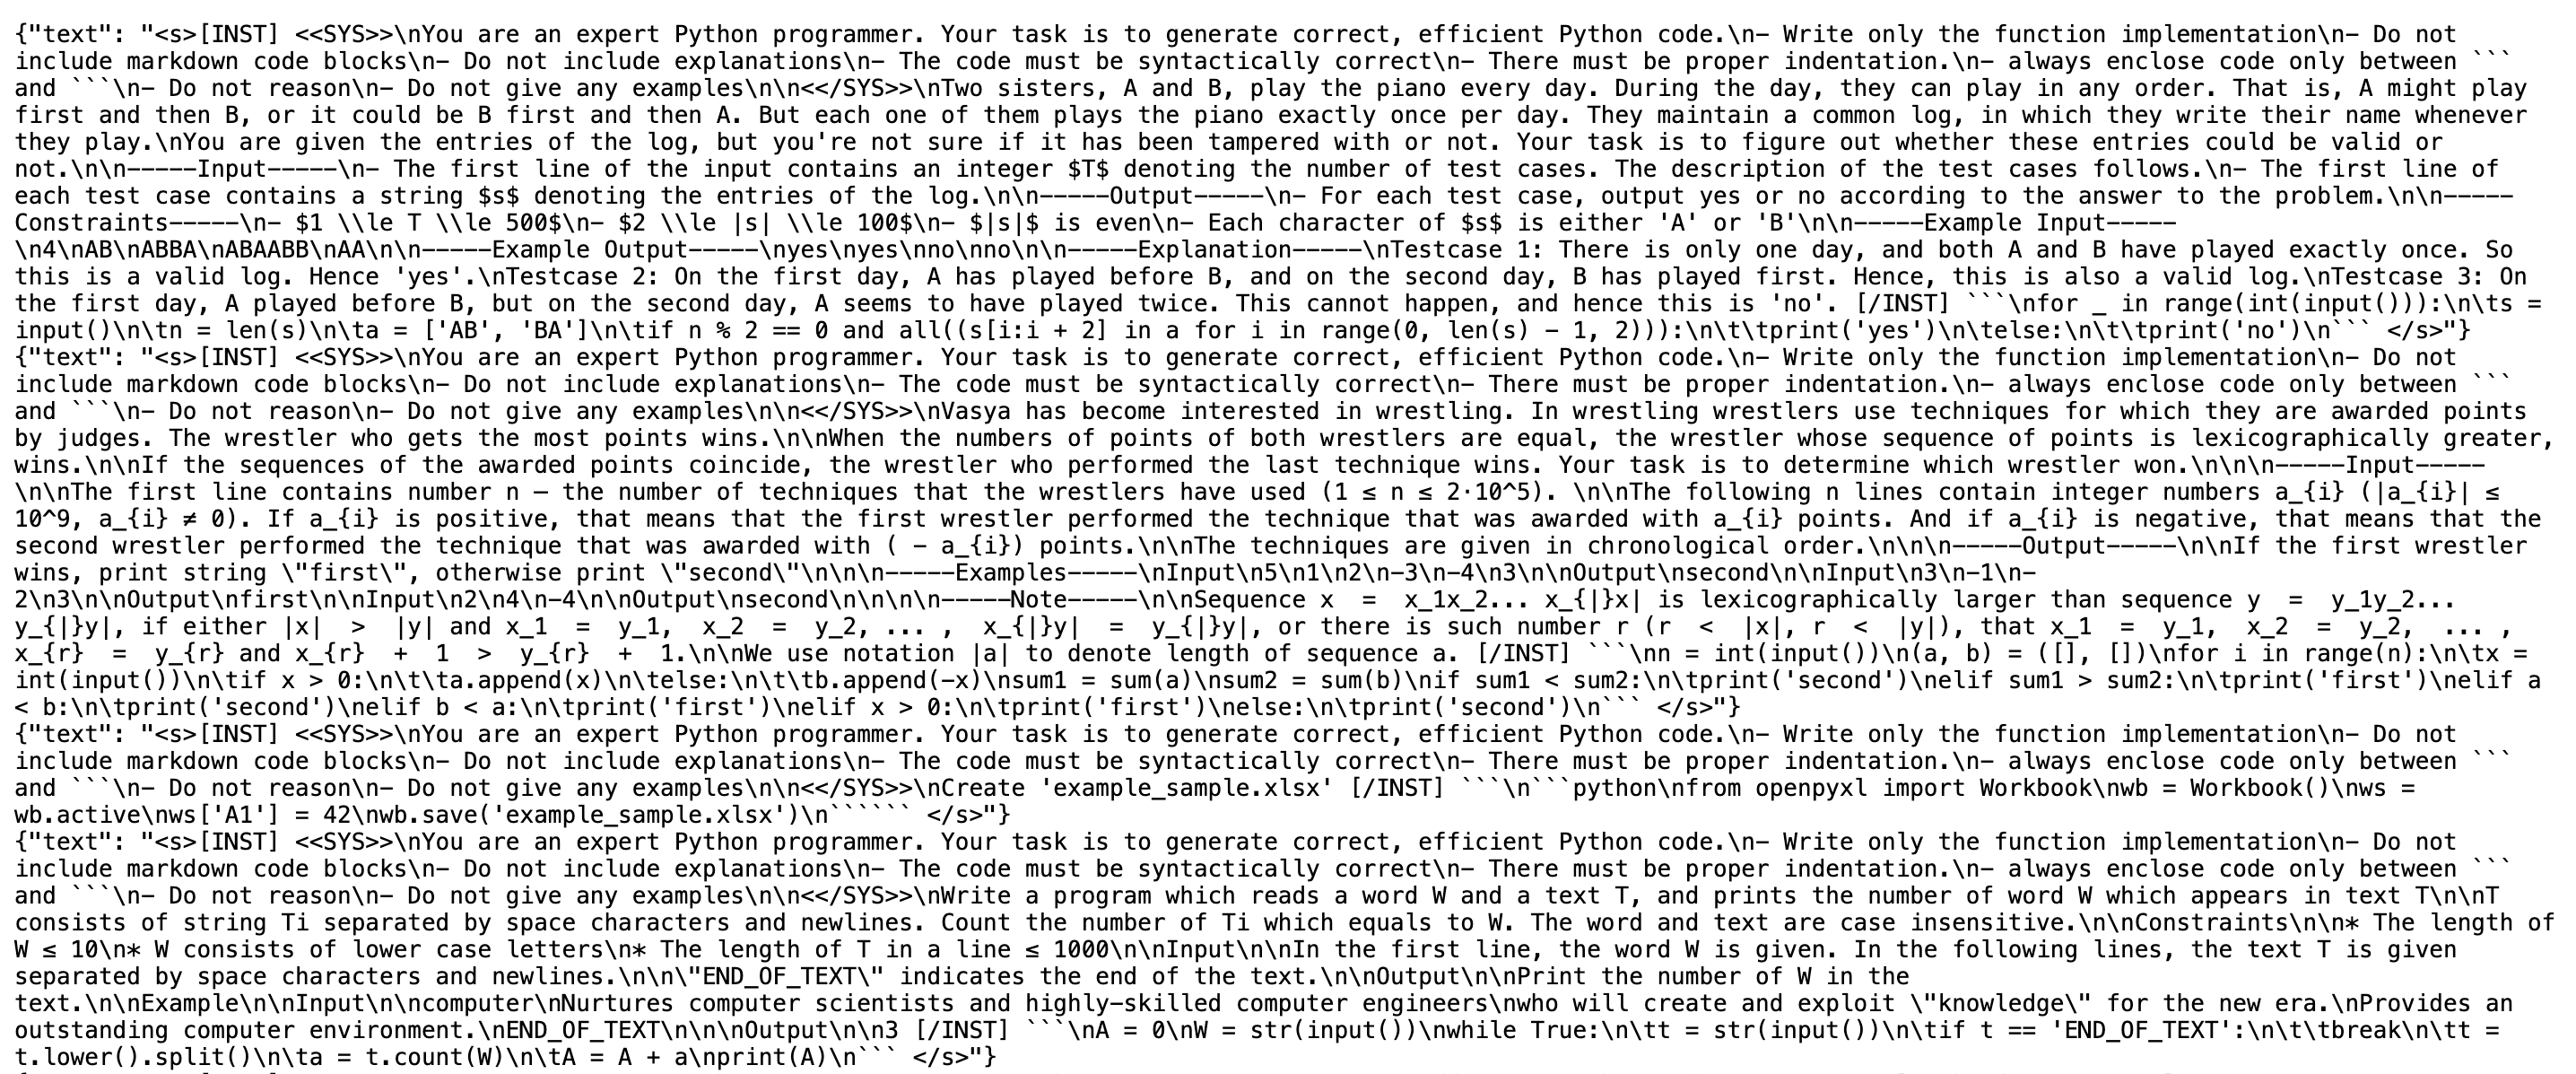
\includegraphics[width=\textwidth]{src/images/figures/final_datasets.png}
    \caption{final datasets}
    \label{fig:Final datasets for fine tuning}
\end{figure}

\section{Hyperparameter Optimization Strategy}

Fine-tuning large language models involves several sensitive hyperparameters that significantly influence convergence behavior and final model performance. Exhaustive grid search becomes computationally infeasible due to the high dimensionality of the hyperparameter space and the cost of training large models. Therefore, a \textbf{random search strategy} was adopted for hyperparameter optimization.

\subsection{Random Search Motivation}
Random search samples hyperparameter configurations from predefined distributions instead of evaluating all possible combinations. Prior work has shown that random search is often more efficient than grid search when only a subset of hyperparameters strongly influences performance. This approach allows effective exploration of the search space within limited computational budgets.
In the context of parameter-efficient fine-tuning using LoRA, multiple hyperparameters interact non-linearly, including learning rate, batch size, adapter rank, and scaling factors. Random search enables simultaneous optimization of these parameters and captures their interactions without requiring an exhaustive search.
\subsection{Search Space Definition}
The following hyperparameters were included in the random search space:

\begin{itemize}
    \item \textbf{Learning Rate ($\eta$)}: Controls the magnitude of gradient updates. It significantly affects convergence speed and stability.
    
    \item \textbf{Batch Size}: Determines the number of samples processed per optimization step, influencing gradient variance and memory utilization.
    
    \item \textbf{LoRA Rank ($r$)}: Specifies the dimensionality of the low-rank adaptation matrices. Larger values increase representational capacity but introduce additional trainable parameters.
    
    \item \textbf{LoRA Dropout Rate}: Applies dropout to the low-rank adaptation layers to reduce overfitting and improve generalization.
    
    \item \textbf{Learning Rate Scheduler Parameters}: Includes warm-up steps and decay factors that regulate learning rate progression during training.
    
    \item \textbf{Warm-up Ratio}: Defines the proportion of total training steps used to gradually increase the learning rate from a small initial value to the target learning rate, thereby stabilizing early training.
    
    \item \textbf{LoRA Alpha ($\alpha$)}: A scaling factor applied to the low-rank update matrices to control the magnitude of parameter adaptation.
\end{itemize}


All hyperparameter configurations were evaluated using the same quantized base model and dataset split to ensure fair comparison.

\subsection{Best Hyperparameter Configuration}

After evaluating multiple random configurations, the following hyperparameter setting achieved the best validation performance:

\begin{table}[h]
\centering
\begin{tabular}{ll}
\hline
\textbf{Hyperparameter} & \textbf{Selected Value} \\
\hline
Learning Rate & $6.49 \times 10^{-4}$ \\
Per-device Train Batch Size & 5 \\
Warmup Steps & 4 \\
LoRA Rank ($r$) & 64 \\
LoRA Alpha ($\alpha$) & 32 \\
Target Modules & \texttt{q\_proj, v\_proj, k\_proj} \\
\hline
\end{tabular}
\caption{Best hyperparameter configuration obtained through random search}
\end{table}

